\documentclass[12pt,a4paper]{article}
\usepackage{listings,chngcntr}
\usepackage{hyperref}% http://ctan.org/pkg/hyperref
\usepackage{paralist}
\usepackage{enumitem}% http://ctan.org/pkg/enumitem
\usepackage{amssymb}
\usepackage{amsmath,amsfonts,bm}
\usepackage{amsthm}
\newtheorem{theorem}{Theorem}[section]
\newtheorem{corollary}{Corollary}[theorem]
\newtheorem{lemma}[theorem]{Lemma}
\usepackage{url}
\usepackage{algorithm}
\usepackage[noend]{algpseudocode}

\makeatletter
\def\BState{\State\hskip-\ALG@thistlm}
\makeatother


\theoremstyle{definition}
\newtheorem{definition}{Definition}[section]
\usepackage{float}
\usepackage[utf8]{inputenc}
\usepackage{cleveref}
\crefname{section}{§}{§§}
\Crefname{section}{§}{§§}
\newcommand{\R}{\mathbb{R}}
 
 \usepackage{graphicx}
 \usepackage{caption}
 \usepackage{subcaption}
 \usepackage[english]{babel}

\usepackage{listings}
\usepackage{color}
\usepackage{graphicx, epstopdf}
\usepackage{listings}
\lstset{language=Python}
\renewcommand{\sectionautorefname}{\S}
\setlength{\topmargin}{0.0in}
\setlength{\oddsidemargin}{0.33in}
\setlength{\textheight}{9.0in}
\setlength{\textwidth}{6.0in}
\renewcommand{\baselinestretch}{1.25}
\setlist[itemize]{noitemsep, topsep=0pt}
\definecolor{codegreen}{rgb}{0,0.6,0}
\definecolor{codegray}{rgb}{0.5,0.5,0.5}
\lstset{
	frame=single,
	numbers = left,
	basicstyle=\fontsize{9}{11}\ttfamily\linespread{0.85}\ttfamily,
    breaklines=true
}
\title{Hierarchical Model Adaptivity}
\author{Author: Georgios Sialounas}

\begin{document}
\counterwithin{lstlisting}{section}
\maketitle
\thispagestyle{empty}
\newpage
\tableofcontents
\setcounter{page}{1}


\section{Introduction and Motivation}
First I will say a few things about the motivation behind the project and motivate adaptivity form both a computational cost and a planet earth perspective.
\subsection{background}
In this section I will present some of the work that has already been done on adaptivity.

\section{Mathematical Formulation}
In this section we present the vectorial Stoke's problem and its formulation in weak form.  
\section{Stoke's Problem}
We consider Stoke's Problem in a domain $\Omega = \left[0,1\right]^2 \subset \mathbb{R}^2$:
\begin{eqnarray}\label{stokes_eq}
	-\Delta\textbf{u} + \nabla p &=& \textbf{f} \\ \label{incomp_eq}
	\nabla\cdot \textbf{u}&=& 0\\ 
\textbf{u}|_{\partial\Omega}&=&0 \label{bc_eq}
\end{eqnarray}
where boldface indicates vectors.  In (\ref{stokes_eq}) and (\ref{incomp_eq}) $\textbf{u},\, f$ and $p$ represent the velocity, the forcing and the pressure respectively.  In this case we have used zero (Dirichlet) boundary conditions. Stoke's equation is used to describe very slow flows (in the limit as the Reynold's number tends to zero).  Such flows might include the motion of the fluid very close to a solid boundary or the flow of magma in the Earth's mantle.  
\subsection{Weak Formulation}
We obtain the weak form of (\ref{stokes_eq}) and (\ref{incomp_eq}) by multiplying the equations with test functions $\textbf{v}$ and $q$ and integrating by parts.  This gives us:
\begin{eqnarray}
	a\left(\textbf{u},\textbf{v}\right) + b\left(\textbf{v},p\right) &=& F\left(\textbf{v}\right)\quad \forall 
\textbf{v} \in \textbf{H}^1_0\left(\Omega\right)^2 \text{ and} \\
	b\left(\textbf{u},q\right)&=&0 \quad \quad\quad\forall q \in L^2\left(\Omega\right),
\end{eqnarray}
where 
\begin{eqnarray}\label{weak-a}
	a\left(\textbf{u},\textbf{v}\right)&=&\int_{\Omega}\nabla \textbf{u} : \nabla \textbf{v}\;\mathrm{d}x \text, \\\label{weak-b}
	b\left(\textbf{v},q\right) &=& \int_{\Omega}-\left(\nabla \cdot \textbf{u}\right)q\;\mathrm{d}x \text{ and}\\\label{weak-F}
    F\left(\text{v}\right) &=& \int_{\Omega}\textbf{f}\cdot \textbf{v} \;\mathrm{d}x.
\end{eqnarray}
An inspection of (\ref{weak-a})-(\ref{weak-F}) will show that we will need $\textbf{u}, \textbf{v}\in \textbf{H}^{1}_{0}\left(\Omega\right)^2$ and $p,\, q \in L^2\left(\Omega\right)$.  Note that we will take the $(\cdot)^2$ in $\textbf{H}^{1}_{0}\left(\Omega\right)^2$ to indicate that we require both components of functions in this space to reside in $\textbf{H}^{1}_{0}\left(\Omega\right)$.
\subsection{Well Posedness}
We will introduce some notation that will be used for the analysis in this section.  We will adopt the same notation as \cite{Chen2016} for ease of cross-checking, as the analysis in this section relies heavily on results presented therein. We firstly reiterate the spaces we will use for the analysis and present the associated norms:
\begin{eqnarray}
\mathbb{V}&=&\textbf{H}^1_0\left(\Omega\right)^2\text{, with norm: } \left|\textbf{v}\right|_{1}=\left|\left|\nabla\textbf{v}\right|\right|_{L^2}, \\
\mathbb{P}&=&\textbf{L}^2_0\left(\Omega\right)=\left\lbrace q\in L^2: \int_\Omega q\;\mathrm{d}x=0\right\rbrace\text{, with norm: } \left|\left|q\right|\right|_{L^2 }
\end{eqnarray}
We will also define two important concepts in terms of proving well-posedness: coercivity and boundedness.
\theoremstyle{definition}
\begin{definition}{Coercivity and boundedness} (see \cite{brenner2007mathematical}: Definition 2.5.2)
	A bilinear form $a\left(\cdot,\cdot\right)$ on a normed linear space $H$ is said  to be bounded (or continuous) if $\exists C\leq \infty$ such that
	\begin{equation}
		\left|a\left(u,v\right)\right|\leq C \left|\left|u\right|\right|_H\left|\left|v\right|\right|_H \quad \forall u,v \in H
	\end{equation}
	and coercive on $V\subset H$ if $\exists$ $\alpha > 0$ such that
	\begin{equation}
	a\left(v,v\right)\geq \alpha \left|\left|v\right|\right|_H^2\quad \forall v \in V.
	\end{equation}
\end{definition}
\subsubsection{PDE}
There are four components to proving the well-posedness for the pde:
	 \begin{eqnarray}\label{coerc_a}
	\inf_{\textbf{u}\in \mathbb{V}}\sup_{\textbf{v}\in \mathbb{V}}\frac{a\left(\textbf{u},\textbf{v}\right)}{\left|\textbf{u}\right| \left|\textbf{v}\right|}&=&\alpha>0,\\\label{coerc_b}
			\inf_{q\in \mathbb{P}}\sup_{\textbf{u}\in \mathbb{V}}\frac{b\left(\textbf{u},q\right)}{\left|\textbf{u}\right|  \left|\left|q\right|\right|}&=&\beta>0,\\\label{cont_a}
		a\left(\textbf{u},\textbf{v}\right)&\leq& C_a\left|\textbf{u}\right|_1\left|\textbf{v}\right|_1,\, \forall \textbf{u},\textbf{v} \in \mathbb{V}\text{ and}\\\label{cont_b}
		b\left(\textbf{u},q\right)&\leq& C_b\left|\textbf{u}\right|_1\left|\left|q\right|\right|,\,\forall \textbf{u} \in \mathbb{V},\, q \in \mathbb{P}.
	\end{eqnarray}
Briefly, (\ref{coerc_a}) and (\ref{coerc_b}) correspond to the stability of the bi-linear forms specified in (\ref{weak-a}) and (\ref{weak-b}) respectively, while (\ref{cont_a}) and (\ref{cont_b}) correspond to their boundedness, in the same order.  It is relatively easier to show that conditions (\ref{weak-a}), (\ref{cont_a}) and (\ref{cont_b}) hold than to show (\ref{weak-b}) holds, so we will start with the latter.  However, firstly we will introduce a result that implies (\ref{weak-b}) holds.  The result can be found in \cite{Chen2016} as Lemma 1.4.
\begin{lemma}\label{Lemma_equiv}
	For any $q\in L^2_0\left(\Omega\right), \exists \textbf{v}\in \textbf{H}^1_0\left(\Omega\right)$ such that
	\begin{equation}
		\nabla \cdot \left(\textbf{v}\right) = q \text{ and } \left|\left|\textbf{v}\right|\right| \lesssim  \left|q\right|.\nonumber 
	\end{equation}
	Consequently, the inf-sup condition, (\ref{coerc_b}), holds.
\end{lemma}
\begin{proof}
	See \cite{Chen2016}: Lemma 1.4
\end{proof}
We will use the statement of \ref{Lemma_equiv} to show that it implies (\ref{coerc_b}).  Consider (\ref{weak-b}).  We choose $\textbf{v}$ so that the result in Lemma (\ref{Lemma_equiv}) holds. We will label this $\textbf{v}$ as $\textbf{v}_q$ to remember the dependence on $q$.   Hence
\begin{eqnarray}
b\left(\textbf{v}_q,q\right) &=& \left|\left|q\right|\right|^2 \quad\text{by Lemma \ref{Lemma_equiv}  and defn of } \left|\left|\cdot\right|\right|,\\
&\gtrsim& \left|\left|q\right|\right| \left|\textbf{v}_q\right|_1\quad \text{by Lemma \ref{Lemma_equiv}},\\
\Rightarrow\frac{b\left(\textbf{v}_q,q\right)}{\left|\textbf{v}_q\right|_1} &\gtrsim& \left|\left|q\right|\right|,\quad \left|\textbf{v}_q\right|_1\neq 0,\\
\Rightarrow \sup_{\textbf{v}\in \mathbb{V}}\frac{b\left(\textbf{v},q\right)}{\left|\textbf{v}\right|_1} &\gtrsim& \left|\left|q\right|\right|,\\
\Rightarrow \inf_{q\in \mathbb{P}}\frac{1}{\left|\left|q\right|\right|}\sup_{\textbf{v}\in \mathbb{V}}\frac{b\left(\textbf{v},q\right)}{\left|\textbf{v}\right|_1} &\gtrsim& 1
\end{eqnarray}
Since $\left|\left|q\right|\right|$ does not depend on $\textbf{v}$, we can move it inside the supremum to obtain the required result, i.e. (\ref{weak-b}) $\qedsymbol$ .  Next, we show that (\ref{coerc_a}) holds.  This is implied by the fact that (\ref{weak-a}) is coercive:
\begin{eqnarray}
		a\left(\textbf{u},\textbf{u}\right)&=&\int_{\Omega}\nabla \textbf{u} : \nabla \textbf{v}\;\mathrm{d}x,\nonumber\\
		&=&\int_{\Omega}\sum_{i}\nabla u_i \cdot \nabla u_i\;\mathrm{d}x\text{ and}\nonumber\\
		&=&\left|\textbf{u}\right|_1^2,\nonumber
\end{eqnarray}
which is the coercivity condition with equality and $\alpha = 1$.  Now we show that  the coercivity of $a\left(\cdot,\cdot\right)$ implies (\ref{weak-a}).  Since $a\left(\cdot,\cdot\right)$ is coercive), we have that
\begin{eqnarray}
a\left(\textbf{u},\textbf{u}\right)&\geq& \alpha  \left|\textbf{u}\right|_1^2 \nonumber \\
\Rightarrow \frac{a\left(\textbf{u},\textbf{u}\right)}{\left|\textbf{u}\right|_1}&\geq& \alpha \left|\textbf{u}\right|_1 \nonumber\\
\Rightarrow  \sup_{\textbf{v}\in \mathbb{V}}\frac{a\left(\textbf{u},\textbf{v}\right)}{\left|\textbf{v}\right|_1} &\geq& \alpha \left|\textbf{u}\right|_1\nonumber\\
\Rightarrow \sup_{\textbf{u}\in \mathbb{V}}\sup_{\textbf{v}\in \mathbb{V}}\frac{a\left(\textbf{u},\textbf{v}\right)}{\left|\textbf{v}\right|_1} &\geq& \alpha>0\nonumber.
\end{eqnarray}
Lastly, (\ref{cont_a}) and (\ref{cont_b}) follow from an application of the Cauchy-Schwarz inequality on the corresponding bilinear forms.
\subsubsection{Discrete form}
Same as for PDE but for discrete case
\subsubsection{Linear System}
In here I will present the linear system arising from the PDE and explain what we will need for it to have a unique solution (I will also show that analysis with the Shur complement etc.)

\section{Adaptivity}
In this section I will explain how I will implement model adaptivity to go from the Stoke's problem to the Poisson problem.

\section{Deal.II}
Deal.II is a C++, open-source, finite element library which we will be using for the implementation of the computatinal aspects of this project.  As a benchmark we will be solving the following problem:
\begin{eqnarray}
\label{benchmark_u}
	\textbf{u}\left(\textbf{x}\right)&=&\begin{bmatrix}
	200x^2\left(1-x\right)^2y\left(1-y\right)\left(1-2y\right)  \\
	-200y^2\left(1-y\right)^2x\left(1-x\right)\left(1-2x\right)  
	\end{bmatrix} \text{ and}\\\label{benchmark_p}
	p &=& 10\left(x-1/2\right)^3y^2+\left(1-x\right)^3\left(y-1/2\right)^3,
\end{eqnarray}
where $\textbf{x}=\left(x,y\right)^T$.    We will substitute (\ref{benchmark_u}) and (\ref{benchmark_p}) as exact solutions (\ref{stokes_eq})to obtain the forcing $\textbf{f}$.  We will use this benchmark example to test for convergence in our model.
\subsection{Computational results}
We are solving (\ref{stokes_eq})-(\ref{bc_eq}) using deal.ii with an adaptive mesh.  Figure \ref{fig_stokes_sol}  shows the magnitude of $\textbf{u}$ plotted at each of 5 refinement cycles required to solve the problem for $\left(\textbf{u}, p\right)$ given by (\ref{benchmark_u}) and (\ref{benchmark_p}).  The convergence results are shown in Table \ref{tablebenchmark_convergence}.
\begin{figure}[H]
	\centering
	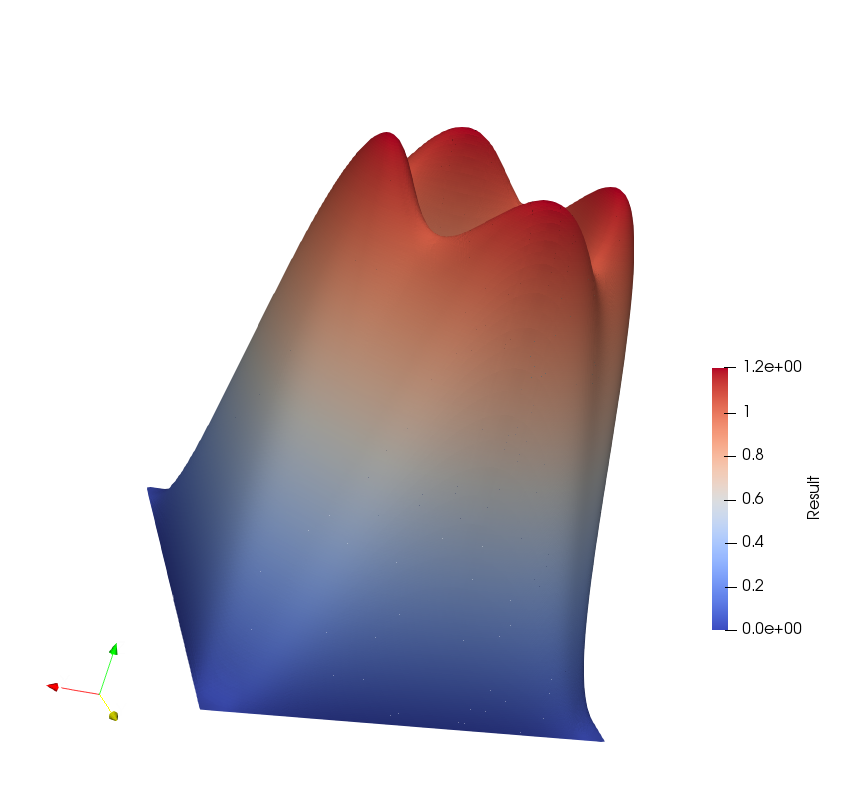
\includegraphics[width=10cm]{stokes_cg_velocities}
	\caption{The magnitude of $\textbf{u}$ plotted at each refinement cycle to (\ref{stokes_eq})-(\ref{incomp_eq}) with $\textbf{u}$ given by (\ref{benchmark_u}).}
	\label{fig_stokes_sol}
\end{figure}
\begin{table}[H]
	\begin{center}
		\begin{tabular}{|c|c|c|c|c|c|} \hline
	refinement cycle & cells & dofs & $||p-p_h||_{L^2}$ & $||u-u_h||_{L^2}$ & $||u-u_h||_{H^1}$\\ \hline
	0 & 64 & 679 & 0.0510 & 0.0108 & 0.4482\\ \hline
	1 & 136 & 1431 & 0.1090 & 0.0099 & 0.4152\\ \hline
	2 & 352 & 3635 & 0.0979 & 0.0071 & 0.2941\\ \hline
	3 & 856 & 8615 & 0.0237 & 0.0010 & 0.0821\\ \hline
	4 & 2128 & 21115 & 0.0120 & 0.0006 & 0.0528\\ \hline
	5 & 5128 & 50427 & 0.0024 & 0.0001 & 0.0151\\ \hline
		\end{tabular}
	\caption{Convergence for $\textbf{u}$ and $p$ in different norms.}
	\label{tablebenchmark_convergence}
	\end{center}
\end{table}
\section{Concluding remarks}
\section{Next steps}
\bibliography{biblio_draft}
\bibliographystyle{ieeetr}
\end{document}